% !TEX encoding = UTF-8
% !TEX TS-program = pdflatex
% !TEX root = ../Tesi.tex
% !TEX spellcheck = it-IT

%************************************************
\chapter{Diagramma E-R}
\label{cap:diagramma}
%************************************************

Una volta analizzate le specifiche del progetto per il quale si vuole realizzare il database, si identificano e si descrivono le singole entità e le loro associazioni.

\section{Descrizione delle entità}
	
	\subsection{Utente}
	
		\begin{figure}[h]
			\centering
			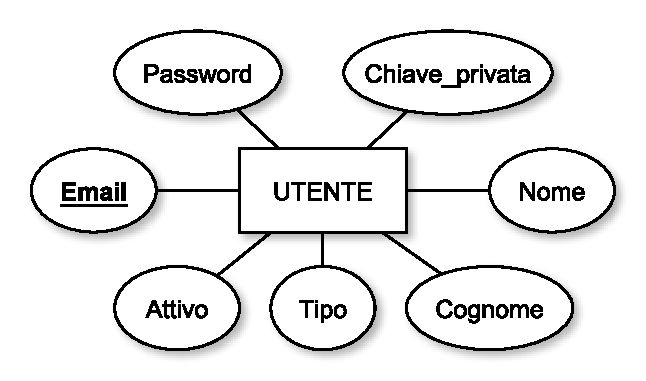
\includegraphics[width=0.5\textwidth]
			{immagini/01-utente}
			
			\caption{Entità Utente}
			\label{entita-utente}
		\end{figure}
		
		Tale entità rappresenta un generico utente dell'applicazione. L'utente si distingue in \emph{Registrato} e \emph{Amministratore}.
		
		La figura \ref{entita-utente} rappresenta l'entità \emph{UTENTE}.
		
		\subsubsection*{Descrizione Attributi}
		
		\begin{description}
			
			\item[Id]
			Chiave primaria dell'entità ``Utente'' che identifica univocamente un utente. Il valore di tale attributo viene inserito dal sistema.
			
			\item[Email]
			Identifica l'email utilizzata dall'utente in fase di autenticazione. Il valore di tale attributo viene inserito dall'utente con relativo controllo di omonimie.
			
			\item[Password]
			Identifica la password utilizzata dall'utente in fase di autenticazione. Il valore di tale attributo viene inserito dall'utente.
			
			\item[Nome]
			Identifica il nome dell'utente con un massimo di 30 caratteri.
			
			\item[Cognome]
			Identifica il cognome dell'utente con un massimo di 30 caratteri.
			
			\item[Tipo]
			Identifica il tipo di utente ovvero:
			\begin{itemize}
				\item
				``A'' per identificare un amministratore;
				\item
				``G'' per identificare il gestore di una squadra;
				\item
				``R'' per identificare un arbitro.
			\end{itemize}
			
			\item[Attivo]
			Identifica lo stato dell'utente, ovvero se è attivo oppure no. Può assumere i valori: ``Y'' oppure ``N''; di default assume valore ``Y'' (attivo).
			
		\end{description}
		
		\subsubsection*{N.B.}
		Nessuno di questi attributi può assumere il valore NULL.
		
		\subsubsection*{Caso Particolare}
		Esiste sempre un valore particolare, ovvero ``admin'', che rappresenta sempre il primo utente Amministratore. Tale valore è sempre presente all'interno della tabella.
	
	\subsection{Amministratore}
	
		\begin{figure}[h]
			\centering
			
\includegraphics[width=0.3\textwidth]
			{immagini/02-amministratore}
			
			\caption{Entità Amministratore}
			\label{entita-amministratore}
		\end{figure}
		
		Tale entità rappresenta la specializzazione dell'entità \emph{Utente}, ereditandone tutti gli attributi. Serve per rappresentare gli utenti \emph{Amministratori}.
		
		La figura \ref{entita-amministratore} rappresenta l'entità \emph{AMMINISTRATORE}.
	
	\subsection{Registrato}
	
		\begin{figure}[h]
			\centering
			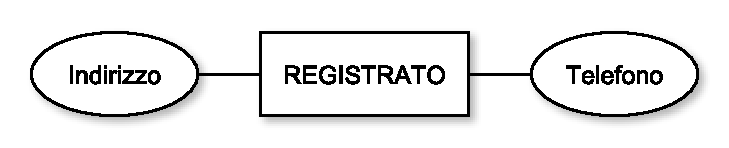
\includegraphics[width=0.6\textwidth]
			{immagini/03-registrato}
			
			\caption{Entità Registrato}
			\label{entita-registrato}
		\end{figure}
		
		Tale entità rappresenta la specializzazione dell'entità \emph{Utente}, ereditandone tutti gli attributi. Serve per rappresentare gli utenti \emph{Gestori Squadra} e gli utenti \emph{Arbitri} che possono accedere all'applicazione Web. Tale entità può essere creata solo dall'amministratore.
		
		La figura \ref{entita-registrato} rappresenta l'entità \emph{REGISTRATO}.
		
		\subsubsection*{Descrizione Attributi}
		
		\begin{description}
			
			\item[Indirizzo]
			Identifica l'indirizzo dell'utente con un massimo di 50 caratteri.
			
			\item[Telefono]
			Identifica il telefono dell'utente con un massimo di 15 caratteri.
			
		\end{description}
		
		\subsubsection*{N.B.}
		Nessuno di questi attributi può assumere il valore NULL.
	
	\subsection{Arbitro}
		
		\begin{figure}[h]
			\centering
			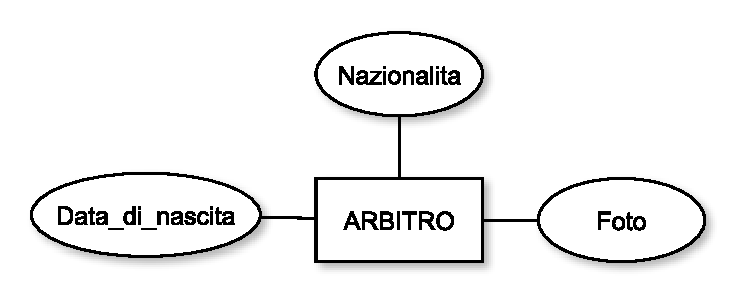
\includegraphics[width=0.6\textwidth]
			{immagini/04-arbitro}
			
			\caption{Entità Arbitro}
			\label{entita-arbitro}
		\end{figure}
		
		Tale entità rappresenta la specializzazione dell'entità \emph{Registrato}, ereditandone tutti gli attributi. Serve per rappresentare il tipo di utente \emph{Arbitro}. Tale entità può essere creata solo dall'amministratore.
		
		La figura \ref{entita-arbitro} rappresenta l'entità \emph{ARBITRO}.
		
		\subsubsection*{Descrizione Attributi}
		
		\begin{description}
			
			\item[Data di nascita]
			Identifica la data di nascita dell'utente.
			
			\item[Nazionalita]
			Identifica la nazionalità dell'utente con un massimo di 50 caratteri.
			
			\item[Foto]
			Identifica il percorso dell'immagine all'interno della cartella \emph{Immagini} del server con un massimo di 50 caratteri.
			
			\item[Carriera]
			Campo utilizzato dall'amministratore per inserire delle informazioni aggiuntive relative all'arbitro.
			
		\end{description}
		
		\subsubsection*{N.B.}
		Nessuno di questi attributi può assumere il valore NULL.
	
	\subsection{Gestore Squadra}
	
		\begin{figure}[h]
			\centering
			
\includegraphics[width=0.3\textwidth]
			{immagini/05-gestore-squadra}
			
			\caption{Entità Gestore Squadra}
			\label{entita-gestore-squadra}
		\end{figure}
		
		Tale entità rappresenta la specializzazione dell'entità \emph{Registrato}, ereditandone tutti gli attributi. Serve per rappresentare il tipo di utente \emph{Gestore Squadra}. Tale entità può essere creata solo dall'amministratore.
		
		La figura \ref{entita-gestore-squadra} rappresenta l'entità \emph{GESTORE SQUADRA}.
	
	\subsection{Torneo}
	
		\begin{figure}[h]
			\centering
			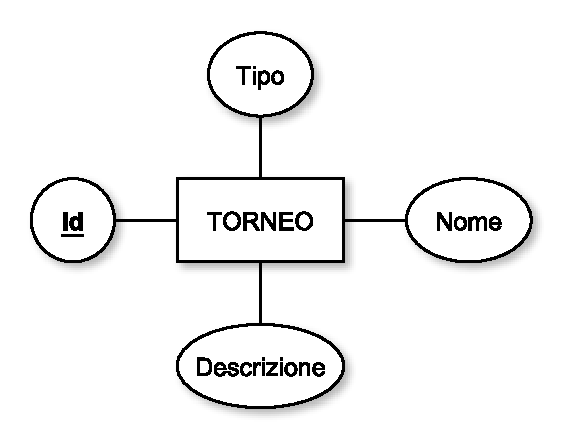
\includegraphics[width=0.5\textwidth]
			{immagini/06-torneo}
			
			\caption{Entità Torneo}
			\label{entita-torneo}
		\end{figure}
		
		Tale entità rappresenta un torneo in svolgimento o già svolto. Può essere di due tipi: ad eliminazione diretta o all'italiana. Tale entità può essere creata solo dall'amministratore.
		
		La figura \ref{entita-torneo} rappresenta l'entità \emph{TORNEO}.
		
		\subsubsection*{Descrizione Attributi}
		
		\begin{description}
			
			\item[Id]
			Chiave primaria dell'entità ``Torneo'' che identifica univocamente un torneo. Il valore di tale attributo viene assegnato automaticamente dal sistema.
			
			\item[Tipologia]
			Identifica la tipologia di torneo ovvero:
			\begin{itemize}
				\item
				``E'' per identificare un torneo ad eliminazione diretta;
				\item
				``I'' per identificare un torneo all'italiana;
			\end{itemize}
			
			\item[Nome]
			Identifica la nazionalità dell'utente con un massimo di 30 caratteri.
			
			\item[Descrizione]
			Campo utilizzato dall'amministratore per inserire delle informazioni aggiuntive relative al torneo (storia, luogo, sponsor, ecc.).
			
		\end{description}
		
		\subsubsection*{N.B.}
		Ad eccezione del campo ``Descrizione'', nessuno di questi attributi può assumere il valore NULL.
	
	\subsection{Partita}
		
		\begin{figure}[h]
			\centering
			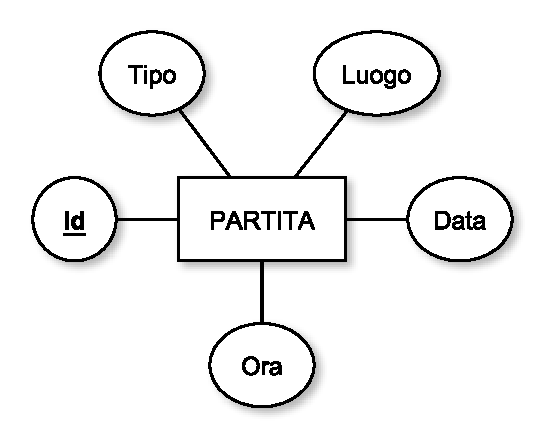
\includegraphics[width=0.5\textwidth]
			{immagini/07-partita}
			
			\caption{Entità Partita}
			\label{entita-partita}
		\end{figure}
		
		Tale entità rappresenta una partita. Tale entità può essere creata solo dall'amministratore.
		
		La figura \ref{entita-partita} rappresenta l'entità \emph{PARTITA}.
		
		\subsubsection*{Descrizione Attributi}
		
		\begin{description}
			
			\item[Id]
			Chiave primaria dell'entità ``Partita'' che identifica univocamente una partita. Il valore di tale attributo viene assegnato automaticamente dal sistema.
			
			\item[Tipo]
			Identifica la tipologia di torneo ovvero:
			\begin{itemize}
				\item
				``E'' per identificare un torneo ad eliminazione diretta;
				\item
				``I'' per identificare un torneo all'italiana;
			\end{itemize}
			Questo attributo serve per gestire in modi diversi le classifiche.
			
			\item[Luogo]
			Identifica il luogo in cui è si svolge la partita con un massimo di 30 caratteri.
			
			\item[Data]
			Identifica la data in cui è si svolge la partita.
			
			\item[Ora]
			Identifica l'ora in cui si svolge la partita.
			
		\end{description}
		
		\subsubsection*{N.B.}
		Nessuno di questi attributi può assumere il valore NULL.
	
	\subsection{Referto}
		
		\begin{figure}[h]
			\centering
			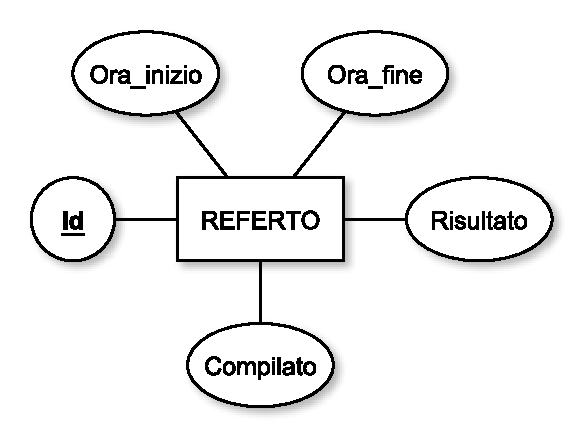
\includegraphics[width=0.5\textwidth]
			{immagini/08-referto}
			
			\caption{Entità Referto}
			\label{entita-referto}
		\end{figure}
		
		Tale entità rappresenta il referto di una determinata gara. Tale entità può essere creata solo dall'arbitro.
		
		La figura \ref{entita-referto} rappresenta l'entità \emph{REFERTO}.
		
		\subsubsection*{Descrizione Attributi}
		
		\begin{description}
			
			\item[Id]
			Chiave primaria dell'entità ``Referto'' che identifica univocamente una partita. Il valore di tale attributo viene assegnato automaticamente dal sistema.
			
			\item[Ora inizio]
			Identifica l'orario effettivo di inizio della partita.
			
			\item[Ora fine]
			Identifica l'orario effettivo di fine della partita.
			
			\item[Risultato]
			Identifica il risultato finale dell'incontro.
			
			\item[Compilato]
			Identifica lo stato del referto, ovvero se è stato compilato oppure no. Può assumere i valori: ``Y'' oppure ``N''; di default assume valore ``N'' (non compilato).
			
		\end{description}
		
		\subsubsection*{N.B.}
		Ad eccezione degli attributi \emph{Ora inizio}, \emph{Ora fine} e \emph{Risultato} tutti gli altri attributi non possono assumere il valore NULL.
	
	\subsection{Squadra}
	
		\begin{figure}[h]
			\centering
			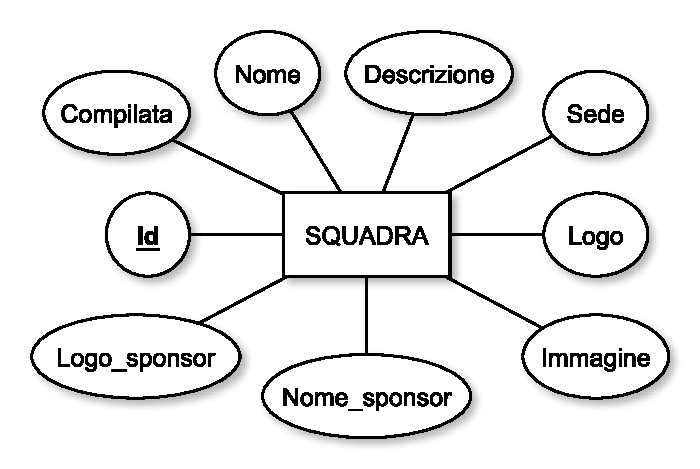
\includegraphics[width=0.6\textwidth]
			{immagini/09-squadra}
			
			\caption{Entità Squadra}
			\label{entita-squadra}
		\end{figure}
		
		Tale entità rappresenta una squadra. Tale entità viene creata dall'amministratore e successivamente viene completata dal gestore della squadra.
		
		La figura \ref{entita-squadra} rappresenta l'entità \emph{SQUADRA}.
		
		\subsubsection*{Descrizione Attributi}
		
		\begin{description}
			
			\item[Id]
			Chiave primaria dell'entità ``Squadra'' che identifica univocamente una partita. Il valore di tale attributo viene assegnato automaticamente dal sistema.
			
			\item[Compilata]
			Identifica lo stato della squadra, ovvero se è stata compilata oppure no. Può assumere i valori: ``Y'' oppure ``N''. Se la squadra non è stata compilata, la prima volta che si accede all'applicazione web si dovranno fornire i dati richiesti. Se non si forniscono i dati della squadra non si può svolgere nessuna attività.
			
			\item[Nome]
			Identifica il nome legale della società con un massimo di 30 caratteri.
			
			\item[Descrizione]
			Campo utilizzato dall gestore della squadra per inserire delle informazioni aggiuntive relative alla squadra.
			
			\item[Sede]
			Identifica la sede legale della società con un massimo di 30 caratteri.
			
			\item[Logo]
			Identifica il percorso del logo della squadra all'interno della cartella \emph{Immagini} del server con un massimo di 50 caratteri.
			
			\item[Immagine]
			Identifica il percorso della foto della squadra all'interno della cartella \emph{Immagini} del server con un massimo di 50 caratteri.
			
			\item[Nome sponsor]
			Identifica il nome dello sponsor ufficiale della squadra con un massimo di 30 caratteri.
			
			\item[Logo sponsor]
			Identifica il percorso del logo dello sponsor all'interno della cartella \emph{Immagini} del server con un massimo di 50 caratteri.
			
		\end{description}
		
		\subsubsection*{N.B.}
		Nessuno di questi attributi può assumere il valore NULL.
	
	\subsection{Classifica}
	
		\begin{figure}[h]
			\centering
			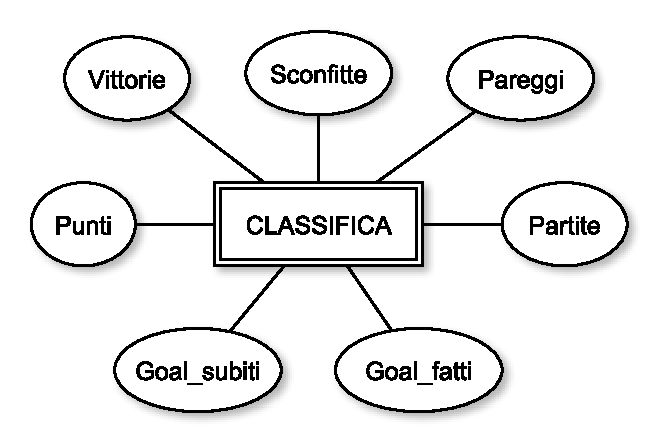
\includegraphics[width=0.6\textwidth]
			{immagini/10-classifica}
			
			\caption{Entità Classifica}
			\label{entita-classifica}
		\end{figure}
		
		Tale entità rappresenta la classifica di un determinato torneo. Tale entità è un'entità debole in quanto non ha propri attributi chiave ma è un torneo ad identificarla univocamente.
		
		La figura \ref{entita-classifica} rappresenta l'entità \emph{CLASSIFICA}.
		
		\subsubsection*{Descrizione Attributi}
		
		\begin{description}
			
			\item[Punti]
			Identifica i punti totalizzati fino a quel momento da una determinata squadra in un determinato torneo.
			
			\item[Vittorie]
			Identifica il numero totale delle partite vinte da una squadra in un determinato torneo.
			
			\item[Sconfitte]
			Identifica il numero totale delle partite perse da una squadra in un determinato torneo.
			
			\item[Pareggi]
			Identifica il numero totale delle partite pareggiate da una squadra in un determinato torneo.
			
			\item[Partite]
			Identifica il numero totale delle partite disputate da una squadra in un determinato torneo.
			
			\item[Goal fatti]
			Identifica il totale dei goal fatti dai giocatori di una determinata squadra in un torneo.
			
			\item[Goal subiti]
			Identifica il totale dei goal subiti dai giocatori una determinata squadra in un torneo.
			
		\end{description}
		
		\subsubsection*{N.B.}
		Nessuno di questi attributi può assumere il valore NULL.
		
	\subsection{Giocatore}
	
		\begin{figure}[h]
			\centering
			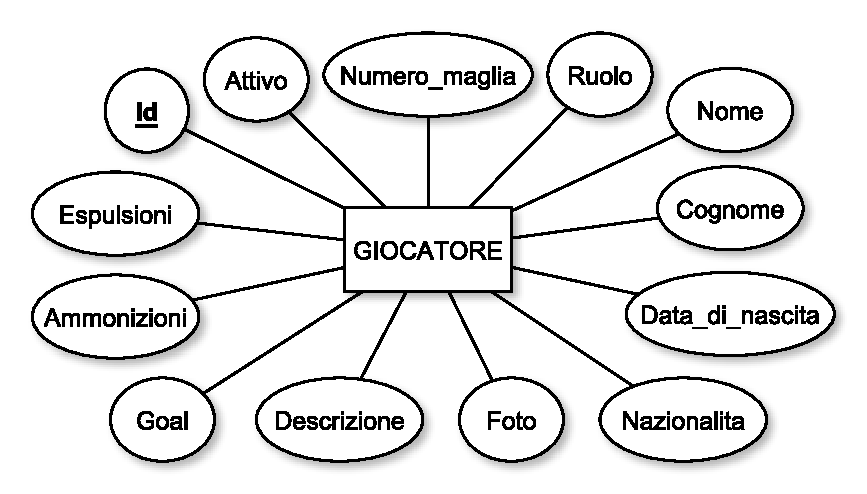
\includegraphics[width=0.8\textwidth]
			{immagini/11-giocatore}
			
			\caption{Entità Giocatore}
			\label{entita-giocatore}
		\end{figure}
		
		Tale entità rappresenta la un determinato giocatore di una squadra.
		
		La figura \ref{entita-giocatore} rappresenta l'entità \emph{GIOCATORE}.
		
		\subsubsection*{Descrizione Attributi}
		
		\begin{description}
			
			\item[Id]
			Chiave parziale dell'entità ``Giocatore'' che identifica univocamente un giocatore appartenente ad una determinata squadra. Il valore di tale attributo viene assegnato automaticamente dal sistema.
			
			\item[Attivo]
			Identifica lo stato del giocatore, ovvero se è attivo oppure no. Può assumere due valori di tipo booleano (true o false); di default assume valore true (attivo).
			
			\item[Numero maglia]
			Identifica il numero maglia con cui il giocatore prende parte alle partite.
			
			\item[Ruolo]
			Identifica il ruolo che il giocatore interpreta in campo con un massimo di 50 caratteri.
			
			\item[Nome]
			Identifica il nome del giocatore con un massimo di 30 caratteri.
			
			\item[Cognome]
			Identifica il cognome del giocatore con un massimo di 30 caratteri.
			
			\item[Data nascita]
			Identifica la data di nascita del giocatore.
			
			\item[Nazionalita]
			Identifica il nome del giocatore con un massimo di 20 caratteri.
			
			\item[Foto]
			Identifica il percorso della foto del giocatore all'interno della cartella \emph{Immagini} del server con un massimo di 50 caratteri.
			
			\item[Descrizione]
			Campo utilizzato dal gestore della squadra per inserire delle informazioni aggiuntive relative al giocatore.
			
			\item[Goal]
			Indica il numero di goal effettuati dal giocatore.
			
			\item[Ammonizioni]
			Indica il numero di ammonizioni del giocatore.
			
			\item[Espulsioni]
			Indica il numero di espulsioni del giocatore.
			
		\end{description}
		
		\subsubsection*{N.B.}
		Nessuno di questi attributi può assumere il valore NULL.

\section{Descrizione delle associazioni}
	
	\subsection{Ha}
	Associazione presente tra Torneo e Classifica.
	L’entità classifica è debole per questo è all'interno di un doppio rettangolo; anche il rombo è doppio per lo stesso motivo. 
	Un entità è debole se non ha attributi chiave; tali entità hanno sempre un vincolo di partecipazione totale perché altrimenti non sarebbero identificabili. Come si può notare è presente un vincolo di partecipazione totale dalla parte di classifica.
	La molteplicità è $1:N$ in quanto ad un torneo sono associate più classifiche (una per ogni squadra), ma una classifica può essere associata soltanto ad un singolo torneo.
	
	\subsection{Presente}
	Associazione presente tra Squadra e Classifica;
	Valgono le stesse considerazioni fatte per la relazione ``Ha''.
	La molteplicità è $1:N$ in quanto ad una squadra possono essere associate più classifiche (una per ogni torneo a cui la squadra partecipa), ma una classifica può essere associata soltanto ad una squadra.
	
	\subsection{Composta}
	Associazione presente tra Squadra e Giocatore.
	Indica quali sono i giocatori che compongono una determinata squadra. In una squadra possono prendere parte al massimo $36$ giocatori. I giocatori possono far parte di una sola squadra. Come si può vedere la molteplicità è $1: 36$.
	I $36$ giocatori sono la rosa della squadra.
	
	\subsection{Gestisce}
	Associazione presente tra Gestore Squadra e Squadra.
	Utile per sapere da chi è gestita una determinata squadra; è presente un vincolo di partecipazione totale dalla parte di squadra in quanto non può esistere una squadra se non esiste un gestore che la crea.
	La molteplicità è $1:1$ in quanto una squadra può essere gestita da un solo gestore e viceversa.
	
	\subsection{Riferito}
	Associazione presente tra Partita e Referto.
	Serve per associare un referto ad una determinata partita che, deve essere o è già stata, giocata.
	È presente un vincolo di partecipazione totale dalla parte di referto in quanto non esiste un referto se non esiste una partita. 
	La molteplicità è $1:1$ poiché ad una determinata partita è associato un solo referto e viceversa.
	
	\subsection{Gestisce Registrato}
	Associazione presente tra Registrato e Amministratore.
	I Registrati del sistema (Arbitri e Gestori squadra) devo essere, creati da uno degli amministratori. Per questo motivo è presente un vincolo di partecipazione totale dalla parte di Registrato. Un Registrato non può esistere se non è presente un Amministratore che lo abbia creato.
	La molteplicità è $1:N$ in quanto un amministratore può creare più utenti Registrati, ma un utente Registrato può essere creato da un solo amministratore.
	
	\subsection{Gestisce Torneo}
	Associazione presente tra Amministratore e Torneo.
	L’amministratore è l’unico a poter creare un torneo (ad Eliminazione diretta o all’Italiana). Per questo motivo è presente un vincolo di partecipazione totale dalla parte di Torneo. Un torneo non può esistere se non c’è un Amministratore che lo abbia creato.
	La molteplicità è $1:N$ in quanto un amministratore può creare molti tornei, ma un torneo può essere creato da un solo amministratore.
	
	\subsection{Compila}
	Associazione presente tra Arbitro e Referto.
	L'Arbitro, prima scelto da un amministratore, sarà colui che ``scrive'' il referto di una specifica partita.
	È presente un vincolo di partecipazione totale dalla parte di referto, in quanto questo non può esistere se non è esiste una arbitro che può compilare tale referto.
	La molteplicità è $1:N$ in quanto un arbitro può compilare $N$ referti ma un solo referto può essere compilato da un solo Arbitro.
	
	\subsection{Partecipa}
	Associazione presente tra Torneo e Squadra.
	Indica a quali tornei partecipano le squadre e quali squadre partecipano ad un determinato torneo.
	La partecipazione totale è dalla parte di torneo perché non può esistere se non sono presenti delle squadre che vi possano partecipare.
	La molteplicità è $M:N$ in quanto una squadra può partecipare a più tornei ed un torneo può avere più squadre che vi partecipano, con un minimo di $2$ per un torneo ad eliminazione diretta e con un minimo di $4$ per un torneo all’italiana.
	
	\subsection{Cartellino}
	Associazione presente tra Arbitro e Giocatore.
	Indica chi sono i giocatori che hanno avuto un ammonizione o un'espulsione dall'arbitro.
	Tale associazione presenta l’attributo Numero che specifica il numero di maglia del giocatore ammonito?
	La partecipazione parziale in entrambe le parti perché può esistere un arbitro che non ha mai assegnato un ammonizione o un'espulsione e, viceversa, giocatore con nessuna ammonizione o espulsione da parte di un arbitro.
	La molteplicità è $M:N$ in quanto un arbitro può ammonire ed espellere più di un giocatore e viceversa.
	
	\subsection{Marcatore}
	Associazione presente tra Referto e Giocatore.
	Indica chi sono i giocatori che hanno segnato un goal in un referto.
	La partecipazione parziale in entrambe le parti perché può esistere un referto con nessun giocatore che ha segnato un goal.
	La molteplicità è $M:N$ in quanto in un referto possono esserci più giocatori che segnano un goal e, viceversa, più giocatore possono segnare più goal.
	
	\subsection{Scelto}
	Associazione ternaria presente tra Arbitro, Amministratore e Partita.
	Indica che un determinato arbitro è stato scelto da un determinato amministratore per una specifica partita.
	Un arbitro può essere scelto per $N$ diverse partite e per ogni partita è scelto un singolo arbitro. Un amministratore può scegliere $N$ arbitri per $N$ diverse partite il ciò vuol dire che un arbitro arbitra una singola partita.
	
	\subsection{Formazione}
	Associazione ternaria presente tra Squadra, Giocatore e Referto.
	Serve per sapere chi sono i giocatori titolari più riserve che faranno parte alla formazione di una determinata partita.
	Nell'associazione è presente un attributo (Riserva) che indica proprio le riserve della partita.
	Se questo è uguale a ``Y'' allora il giocatore scelto sarà una riserva, in caso sia ``false'' il giocatore sarà un titolare.
	Per ogni referto sono fornite due formazioni, una per ogni squadra, composte da 18 giocatori ($11$ titolari e $7$ riserve).
	
	\subsection{Giocano}
	Associazione ternaria presente tra Partita, Torneo e Squadra.
	Indica quali squadre di un determinato torneo si devono affrontare. Tale associazione presenta l’attributo Nome\_partita che specifica il nome della fase o il nome della giornata dei tornei rispettivamente ad eliminazione diretta o all'italiana. Una partita viene giocata sempre da $2$ squadre e fa parte di un singolo torneo, in un torneo sono possibili $N$ partite. C’è un vincolo di partecipazione totale dalla parte di partita in quanto essa non può esistere se non è stato creato un torneo o sono presenti delle squadre.
	

\section{Il modello E-R completo}
Per il modello E-R completo si veda la figura \vref{fig-modello-ER}.


\begin{figure}[h]
	\centering
	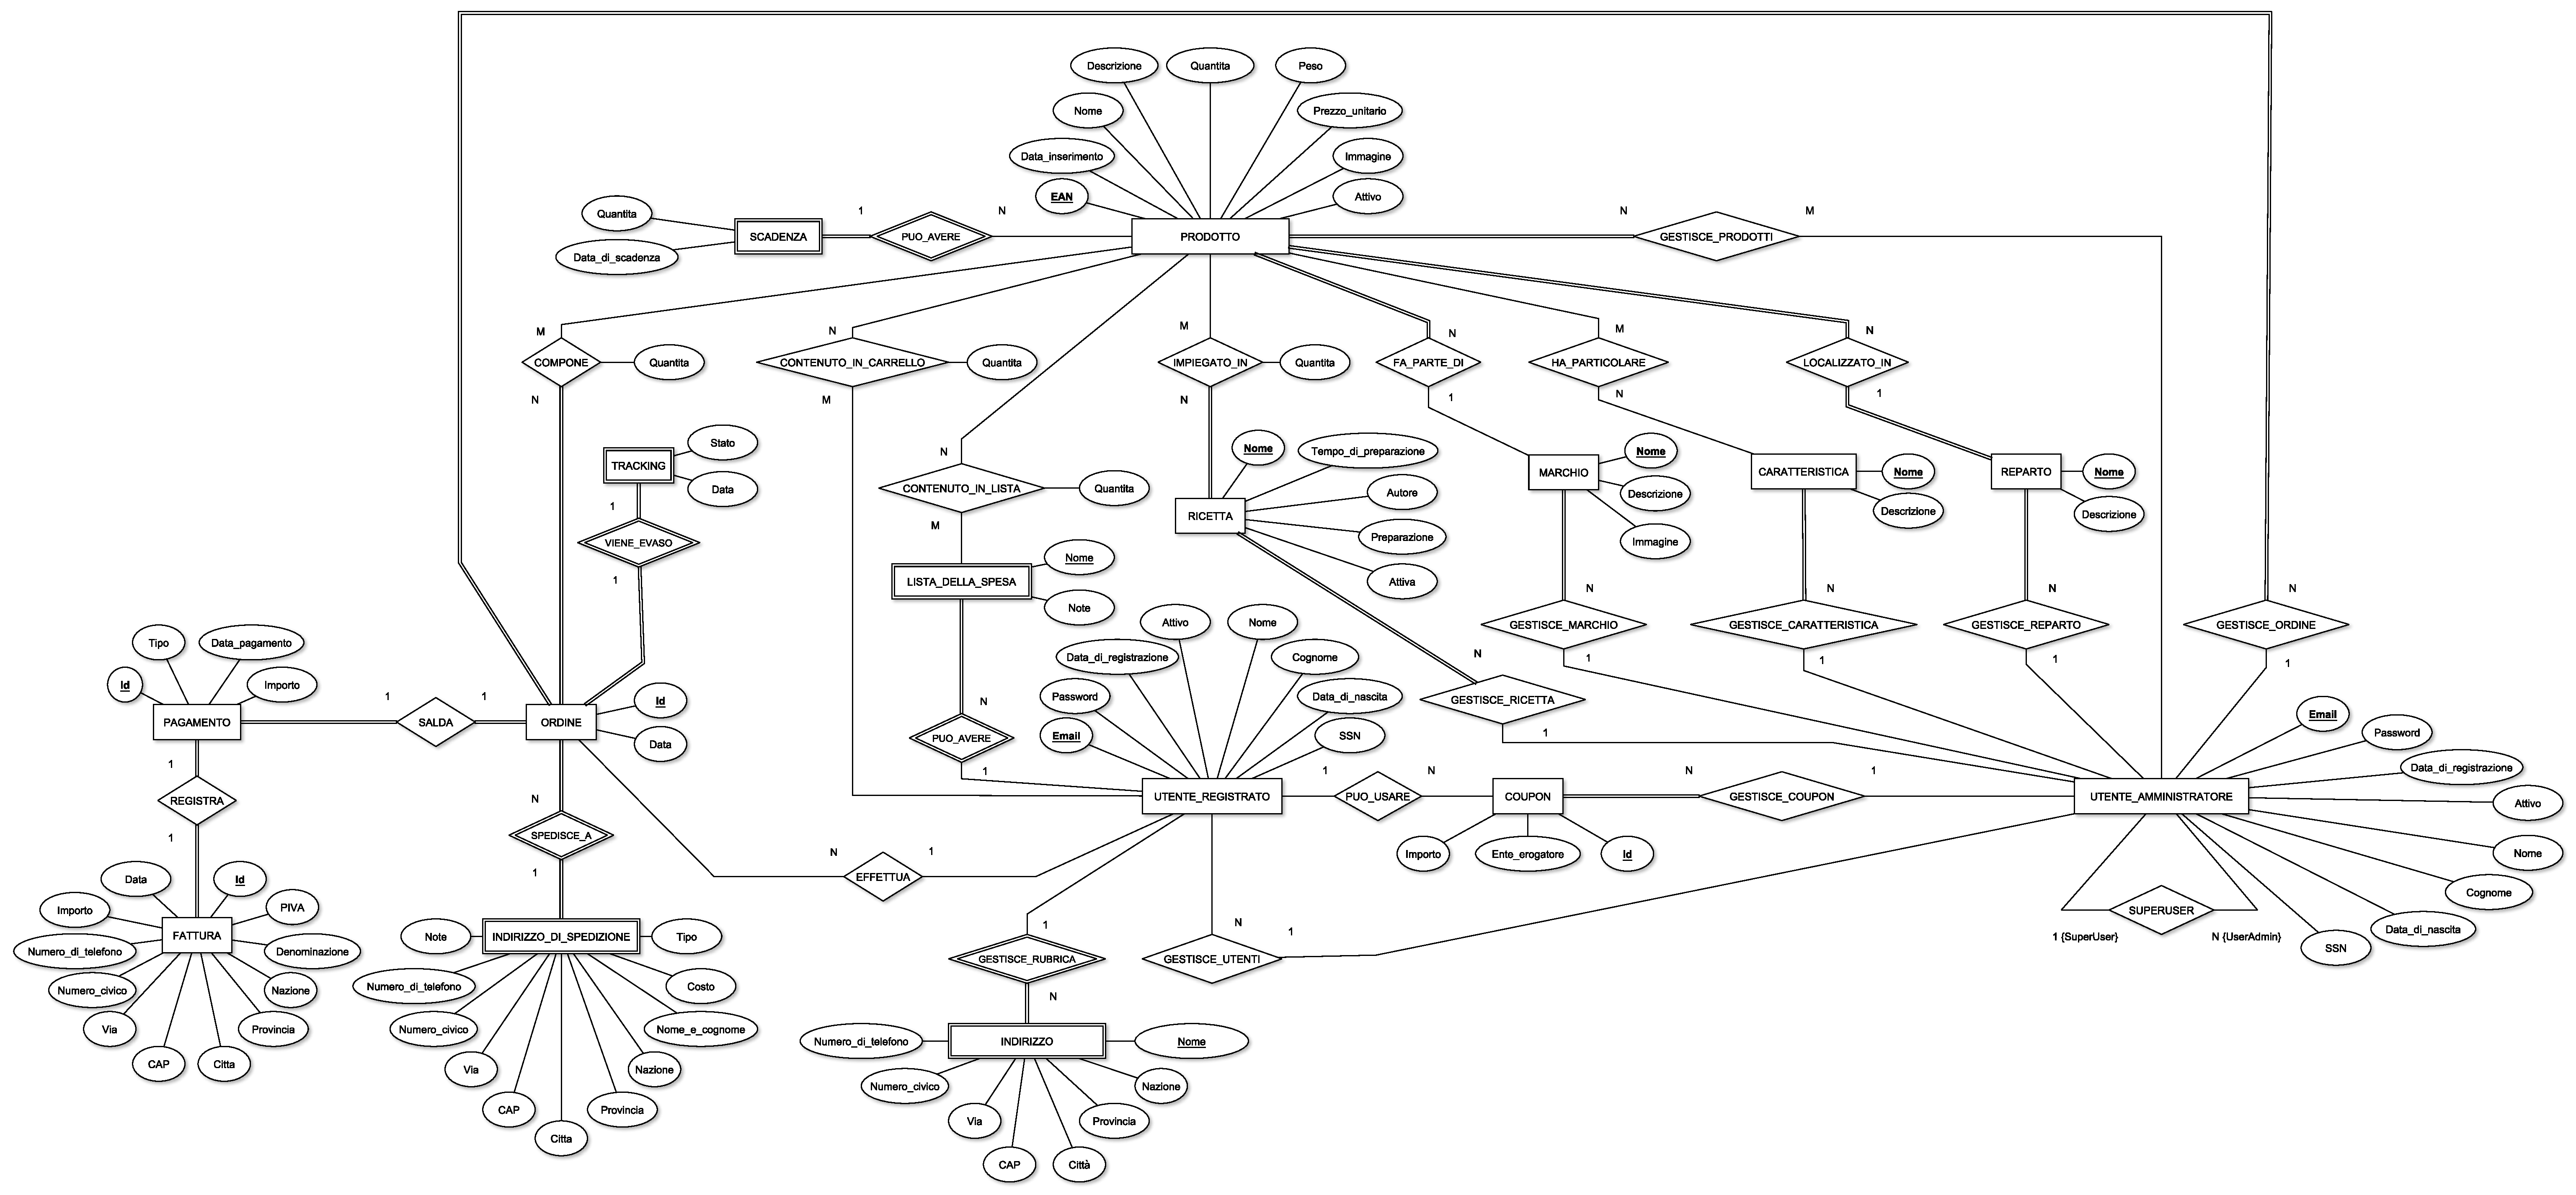
\includegraphics[height=0.83\textwidth,
	angle=90]
	{immagini/diagramma-ER-completo}
	
	\caption{Schema E-R completo}
	
	\label{fig-modello-ER}
\end{figure}	